%!TEX root = ../Thesis.tex

\chapter{Grundlagen}
\label{cha:grundlagen}

In diesem Kapitel werden die für das Verständnis und die Durchführung der Arbeit benötigten
Grundlagenthemen vorgestellt. Nach einer kurzen Erläuterung der Möglichkeiten der Verkehrsanalysen
mittels Luftaufnahmen, wird daher darauf eingegangen, auf welche Weise die in dieser Arbeit verwendeten
Fahrzeugtrajektorien ermittelt werden.
Anschließend werden Methoden vorgestellt, welche zur Bereinigung der gewonnenen Daten verwendet werden können.
Als wichtiges Mittel zur Identifizierung von Fahrspuren aus Trajektorien werden zudem
verschiedene Cluster-Algorithmen und Distanzmaße vorgestellt. 

\section{Verkehrsanalyse mittels Luftaufnahmen}
\label{sec:traffic_analysis}

% Beschreibung der Aus den Luftaufnahmen ermittelten (ermittelbaren) Werte
% Vorteile der Verwendung von Luftaufnahmen zur Erstellung von Verkehrssimulationen 

\section{Rekonstruktion von Fahrzeugtrajektorien aus Luftaufnahmen}
\label{sec:position_extraction}

% Beschreibung des kompletten Vorgangs bis Bewegungsbahnen der Autos vorliegen
% Tracking --> World-Matching --> Glättung

Die in dieser Arbeit verwendeten Fahrzeugtrajektorien stammen aus der Anwendung ``Tracker-Application''
des MEC-View Teilprojektes \textit{Luftbeobachtung}. Nachfolgend wird beschrieben, wie diese aus den Videoaufnahmen
rekonstruiert werden.

Die Verfolgung von bewegten Objekten beziehungsweise Fahrzeugen, wird in der ``Tracker-Application'' mittels
\textit{Supervised Tracking} umgesetzt. Bei diesem Verfahren wird ein initial manuell ausgewählter Bildbereich
automatisch mit Hilfe eines erlernten Klassifikators verfolgt. Der Klassifikator muss hierbei zwischen
Fahrzeugen und der Umgebung unterscheiden können.
Das grundlegende Vorgehen dieses Tracking-Ansatzes ist in Abbildung \ref{fig:grund_tracking}
dargestellt und kann wie folgt beschrieben werden:

\begin{itemize}
    \item[a)] Verfolgtes Objekt befindet sich zum Zeitpunkt $t$ an bekannter Position $p_1$
    \item[b)] Zum Zeitpunkt $t+1$: Anwendung des Klassifikators auf Positionen um $p_1$
    \item[c)] Erstellen einer \textit{Confidence Map}, welche die Wahrscheinlichkeit darstellt, das verfolgte Objekt gefunden zu haben
    \item[d)] Updaten des Trackers auf Position des Maxima der \textit{Confidence Map}
\end{itemize}

\begin{figure}[H]
    \centering
    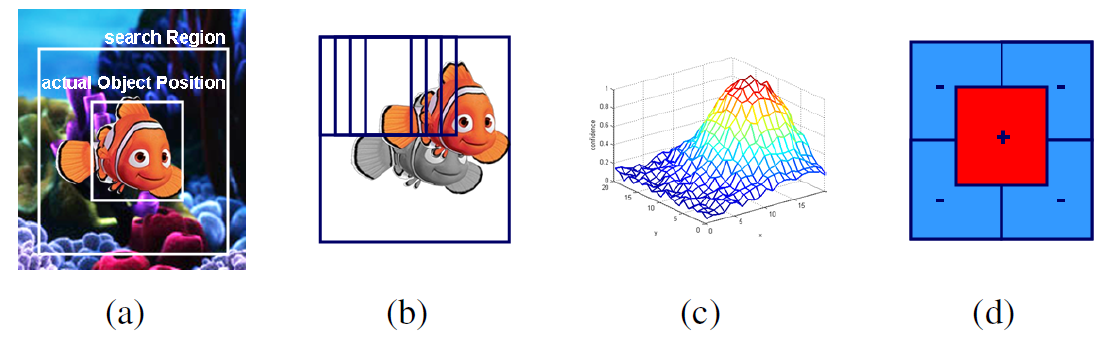
\includegraphics[width=0.7\linewidth]{../resources/img/grundlagen/tracking}
    \caption[Übersicht Tracking mit Klassifikator]{Übersicht Tracking mit Klassifikator [\cite{Grabner}]}
    \label{fig:grund_tracking}
\end{figure}

Das Erlernen eines stabilen Klassifikators in der ``Tracker-Application'' basiert auf der Arbeit
\textit{``Real-Time Tracking via On-line Boosting''} von \cite{Grabner}.
Die Autoren verwenden einen On-line AdaBoost Algorithmus, welcher mehrere \textit{schwache}
Klassifikatoren zu einem \textit{starken} Klassifikator kombiniert.
Schwache Klassifikatoren müssen hierbei nur eine Erkennungsrate von mehr als 50\% besitzen und somit
wenig besser als zufallsbedingtes Auswählen sein.
Starke Klassifikatoren entstehen durch die Kombination von mehreren schwachen Klassifikatoren.
Die Auswahl von schwachen Klassifikatoren erfolgt über sogenante Selektoren, welche aus einem Set
von schwachen Klassifikatoren immer jenen auswählen, welcher die geringste Fehlerrate bei der Erkennung
der Trainings-Objekte besitzen. Der Klassifikator mit der schlechtesten Erkennungsrate wird in jeder
Trainingsiteration ersetzt, um das Training weiter zu verbessern.

\section{Datenaufbereitung und Bereinigung}
\label{sec:tra_preprocessing}

% ALLGEMEINE Beschreibung von möglichen Datenbereinigungsschritten
% Resampling (Distanz oder Geschwindigkeit)
% Padding etc. (Interpolation)
% Glättung (RANSAC, Wavelet)

\section{Clusteranalyse von Trajektorien}
\label{sec:tra_clustering}

\subsection{Clustering Algorithmen}
\label{sec:cluster_algos}

\subsection{Distanzmaße zum Vergleich von Fahrzeugtrajektorien}
\label{sec:distance_measures}

\section{Untersuchung von möglichen Straßentopologien}
\label{sec:street_topologies}